\section{(Basic) Predicting ELMs in proteins}
\label{sec:predicting_p53}

One of the most useful (and used) features in ELM is the ability to
detect motifs in proteins and sequences. Given a protein's amino acid
sequence, the ``EML Predictions'' pipeline searches for occurrences of
each motif class using regular expressions, apply a set of filters to
help judging results, and to visualize resulting set of putative motifs.

In this protocol we will be viewing the manually annotated data of a
typical protein, using p53 (Uniprot ID: P53\_HUMAN/P04637) as an
example. We will cover how to find the manually annotated motifs and
instances, and how to find the motif instances, the references used to
annotate each instance, the experimental protocols used, and additional
information including relationships to biological pathways (KEGG), diseases
(OMIM) and molecular switches (from switches.ELM)

TODO: MARC: check the above text

%
% Subsection: Necessary Resources
%

\subsection{Necessary Resources}\label{necessary-resources}

\subsubsection{Software \& Hardware}\label{software-hardware}

A modern browser such as Firefox, Chrome, or Safari. ELM is best viewed
on a laptop or desktop computer, although tablets and smartphones will
also work.

\begin{enumerate}

%
% Subsection:Predicting ELM insstances
%

\subsection{Predicting ELM instances: Input form}
\label{subsec:predicting_p53_input}

\begin{figure}[h!]
	\centering
	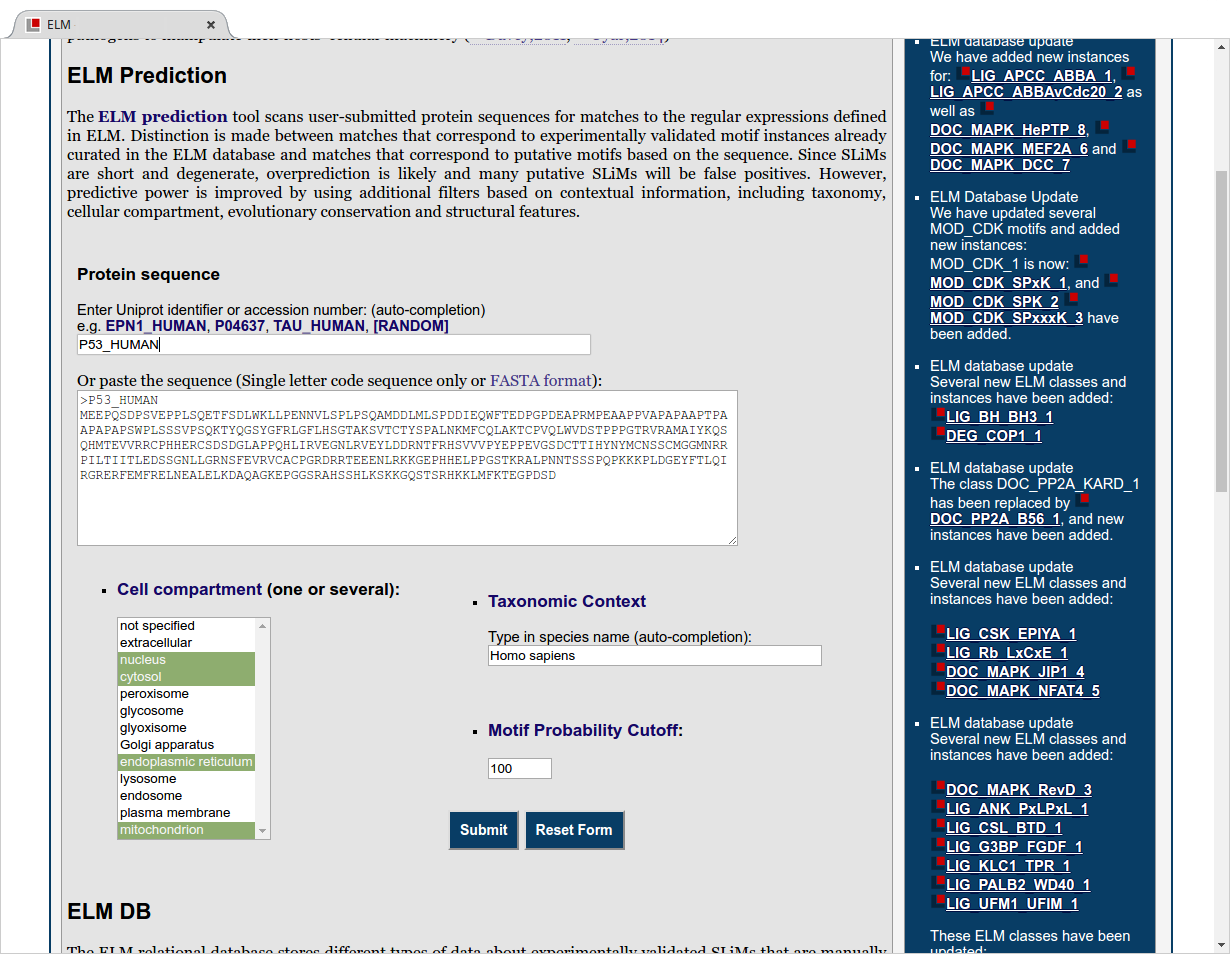
\includegraphics[width=\textwidth]{Figures/predicting_p53/elm_search.png} 
	\caption{
	The ELM input page for predicting motifs in a protein.
	}
	\label{fig:predicting_p53_elm_search}
\end{figure}

\item Open a browser, and navigate to the ELM homepage: http://elm.eu.org.
	Enter the Uniprot ID \uniprot{P53\_HUMAN} in the search field labelled
	``Enter a uniprot identifier or accession number''. The page should
	autocomplete/suggest the protein ``\uniprot{P53\_HUMAN} / P04637 (Homo
	sapiens)'' (Fig. \ref{fig:predicting_p53_elm_search}).
	Click on this entry to confirm that we want to search for
	motifs in this protein. Click on \button{Submit} to submit the query to
	the server.

	\sdesc{The autocompletion mechanism queries Uniprot for protein
		identifier; if it succeeds, then additional information from
		Uniprot will be used to pre-populate the filter boxes. In this
		example, \uniprot{P53\_HUMAN} is recognized as a Human protein,
		and so ``Homo sapiens'' is automatically filled in the
		``Taxonomic Context'' field. Also, P53 has been annotated (by
		Uniprot) to be localized to nucleus, cytosol, endoplasmic
		reticulum and mitochondrion, so these are also automatically
		applied as search criteria. The motif cutoff of ``100'' is a
		sufficiently high (lenient) threshold to allow all other
		detected motifs to be shown.}

\item Select the search criteria (optional). It is possible to limit the
	results by ``cell compartment'', ``taxonomic context'' or by changing
	the ``motif probability cutoff''. To restrict the search to include
	motifs that are active in certain cellular compartments, select one or
	more from the list (use the ``control'' key to select more than one
	option). It is also possible to select a ``taxonomic context'' to
	restrict the search to motifs from certain species. Start typing a
	species name in the ``taxonomic context'' input field to get an
	auto-completed list of species to select from. Additionally, a ``Motif
	probability cutoff'' can be used to only retain ELM classes whose
	pattern probability is below the given value. For the current protocol,
	leave all of these at their default values: ``not specified'', ``100''
	and no ``taxonomic context''

TODO: Repeat search using stringent filters (homo sapiens, nucleus,
0.01) Do we want to do this? - Marc

%
% Subsection: Interpreting results: graphical summary
%

\subsection{Interpreting the prediction results: Graphical Summary}
\label{subsec:predicting_p53_graphical_summary}

\item Click \button{submit} to start searching for motifs. You will be brought
	to an intermediate page indicating that your results are being
	processed, and should be redirected to the final results page
	within a minute. You can bookmark this page: The results are stored for
	a week.

	\sdesc{The Results are summarized in the first figure on the results
		page (see figure \ref{fig:predicting_p53_results_summary}).
		The graphical summary shows the
		results generated by the ELM prediction pipeline, combined with
		additional filters and information from external resources. The
		visualization should help you interpreting the results and to
		assess whether or not a motif is present in a sequence, as well
		as how likely it is to be functional based on its structural
		context and evolutionary conservation. Motif instances which
		are manually annotated in the database appear as red (TP) or
		yellow (FP) ovals in the graphic. Blue/gray squares represent
		predicted motif occurrences.}

\begin{figure}[h!]
	\centering
	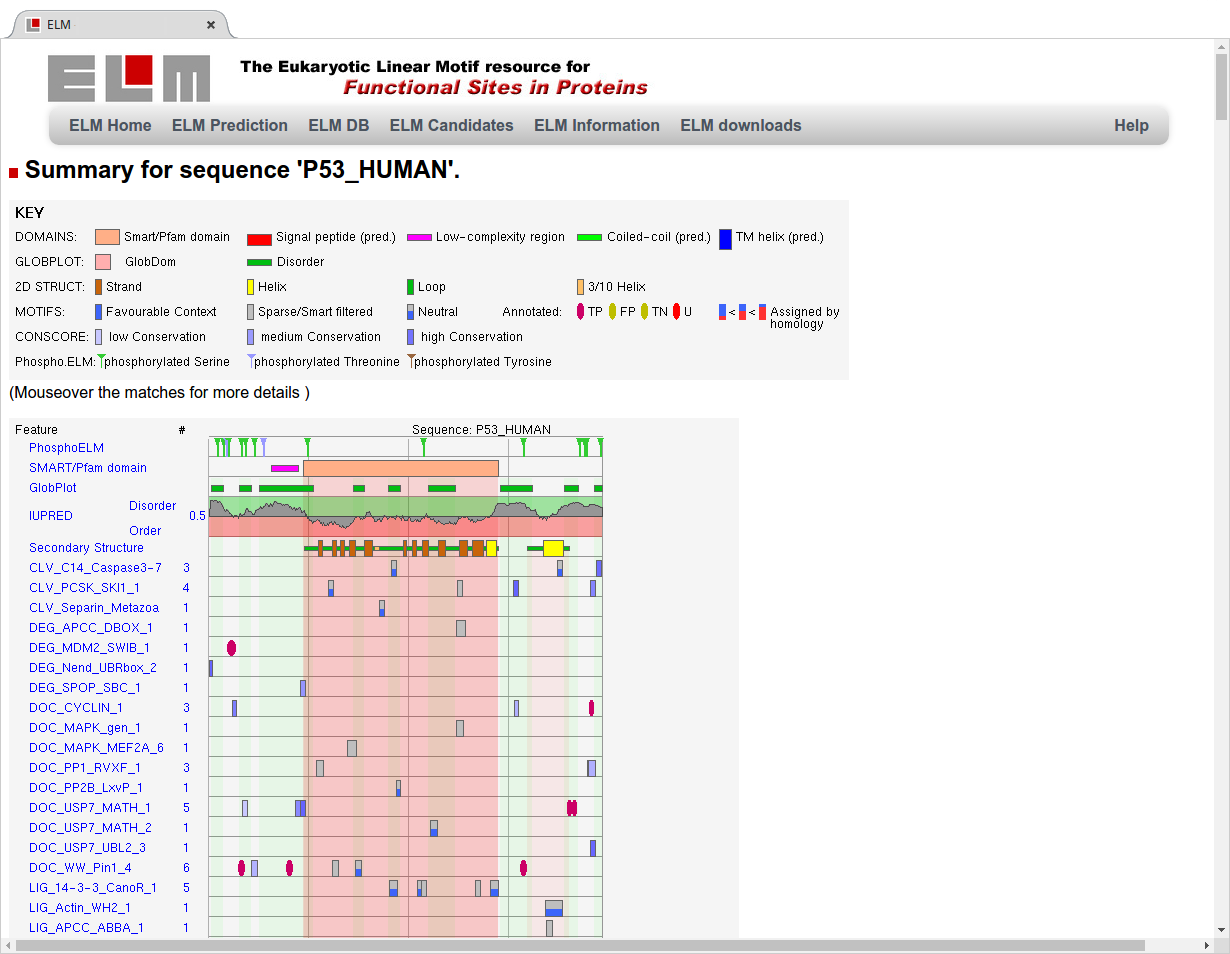
\includegraphics[width=\textwidth]{Figures/predicting_p53/elm_results_summary.png} 
	\caption{
	The graphical results summary of the ELM Prediction pipeline for
	\uniprot{P53\_HUMAN}. Note that not all motif detections are shown (the
	image is truncated at the bottom). The top five rows show a set of
	structural features. Annotated and predicted motifs are shown as
	differently colored ovals/boxes. The info screens for two motifs are
	shown: \motif{CLV\_C14\_Caspase3-7} and \motif{CLV\_PCSK\_SKI1\_1}.
	}
	\label{fig:predicting_p53_results_summary}
\end{figure}

\item The first row contains phosphorylation sites as retrieved from
	phospho.ELM \cite{21062810}, and whether the phosphorylated amino
	acid is a serine, threonine or tyrosine. Phospho.ELM is a database of
	manually annotated phosphorylation sites obtained from scientific
	publications from low and high-throughput experiments. You can follow
	the link to phospho.ELM by clicking on the phosphorylation site in the
	image to get more information on individual phosphorylation sites.

	\sdesc{Phosphorylation sites are only available when the search is
		performed with a protein accession (eg. \emph{not} with a FASTA
		sequence alone) in step 1 and there is relevant information
		annotated in the phospho.ELM database. Phosphorylation sites
		are relevant to interpret ELM motif predictions when the
		predicted motif requires to be phosphorylated (as in several
		docking and ligand binding motifs) and for predicting 
		phosphorylation motifs.}

\item The second row shows SMART and Pfam domains detected by the SMART
	database \cite{9600884, 25300481, 9600884}
	(Fig. \ref{fig:predicting_p53_results_summary}). Hover the
	mouse over these domains to see their names and exact start and end
	positions.

	\sdesc{ In order to be functional motifs to be accessible, and
		therefore they are usually not found within globular domains
		and structured regions (\cite{21909575}). Any motifs detected
		by the ELM prediction pipeline inside of a smart domain are
		less likely to be functional, and are shown as a gray box
		background (see also the ``structural filter'' described in
		step XXX). }

\item The third row shows globular and disordered regions in the
	sequence as predicted by GlobPlot (\cite{12824398}). The fourth
	and fifth rows
	contain results from IUPred (\cite{15955779}), another
	predictor of disordered protein regions. Protein segments with
	an IUPred score above 0.5 are considered to be disordered.

	\sdesc{Motifs are typically only functional when found in intrinsically
		disordered regions. Any motif occurrence detected by the ELM
		prediction pipeline that falls within disordered regions are
		more likely to be functional.}

\item The 5th row (Fig. \ref{fig:predicting_p53_results_summary}) contains
	information on secondary structure. The secondary structure is
	predicted using a pipeline mapping motif occurrence onto high quality
	reference domain structures \cite{19852836}. Check the graphical
	representation, and if the output of the secondary structure filter and
	the disorder predictors agree with respect to which parts of the
	sequence are considered structured and which disordered.

\item The remainder of the figure (below ``secondary structure'' output)
	displays predicted and annotated motif instances, overlayed with the
	structural context from rows 2 and 3 (SMART domains and GlobPlot). A
	blue square indicates a single motif occurrence, and intensity of the
	color indicates the conservation of this sequence across a group of in
	homologous proteins.
	Boxes in gray are motif occurrences which have been filtered out by the
	structure filter. Boxes that are blue \& gray are neutral (
	residing in structural context, but the secondary structure detected a
	loop region). If the sequence is already present in the ELM database,
	any motif instances that have already been annotated are shown as
	ovals. Lastly, any motifs detected which are annotated to be
	functional in homologous sequences, are shown as red \& blue
	rectangles.

	\sdesc{ In the case that not enough homologous sequences were detected
		to build an alignment, no conservation score can be calculated.
		Therefore all of the motif occurrences will be shown in a
		uniform shade of blue. }

TODO: EXPLAIN / SHOW ANNOTATED INSTANCES Marc: Use mouse over in this figure.

\item Place the cursor over the blue box for motif occurrence 
	\motif{CLV\_C14\_Caspase3-7} at the end of the sequence (
	position 388-392). This will trigger the green and yellow 
	information screen shown on the top right in Fig.
	\ref{fig:predicting_p53_results_summary}.
	This motif is in a disordered region, and has not been
	filtered out by the structural filter. Also, its conservation score
	of 0.910 is very high, indicating that this motif is highly conserved.

	\sdesc{The confidence score is based on how conserved the sequence is
		across a set of homologous proteins from other sequences. An
		full description of the method can be found in \cite{18460207}.
		The higher the conservation score (max. 1), the more conserved
		the motif's sequence is, and the more likely it is a functional
		motif for this prediction.}

\item Place the cursor over the blue \& gray rectangle for motif
	\motif{CLV\_PCSK\_SKI1\_1} at position 120-124, a motif 
	which was flagged as ``neutral'' by the ELM prediction pipeline.
	This will trigger the information screen (with the pink header) shown
	in Fig. \ref{fig:prediction_p53_results_sumamry} to appear.
	This motif resides inside of the P53 Pfam domain, and thus has been
	subjected to ``structural filtering''. However, the secondary structure
	prediction suggests this motif occurs within the looped regioun of this
	domain, so may be accessible.

	\sdesc{The information screen pop-up 
	shows scores for all of the individual criteria used by the secondary
	structure filter: The name of the domain, the \emph{accessibility
	score} , \emph{secondary structure score}, \emph{combined total score},
	and the associated \emph{total score P-value} \cite{19852836}.}

\begin{figure}[h!]
	\centering
	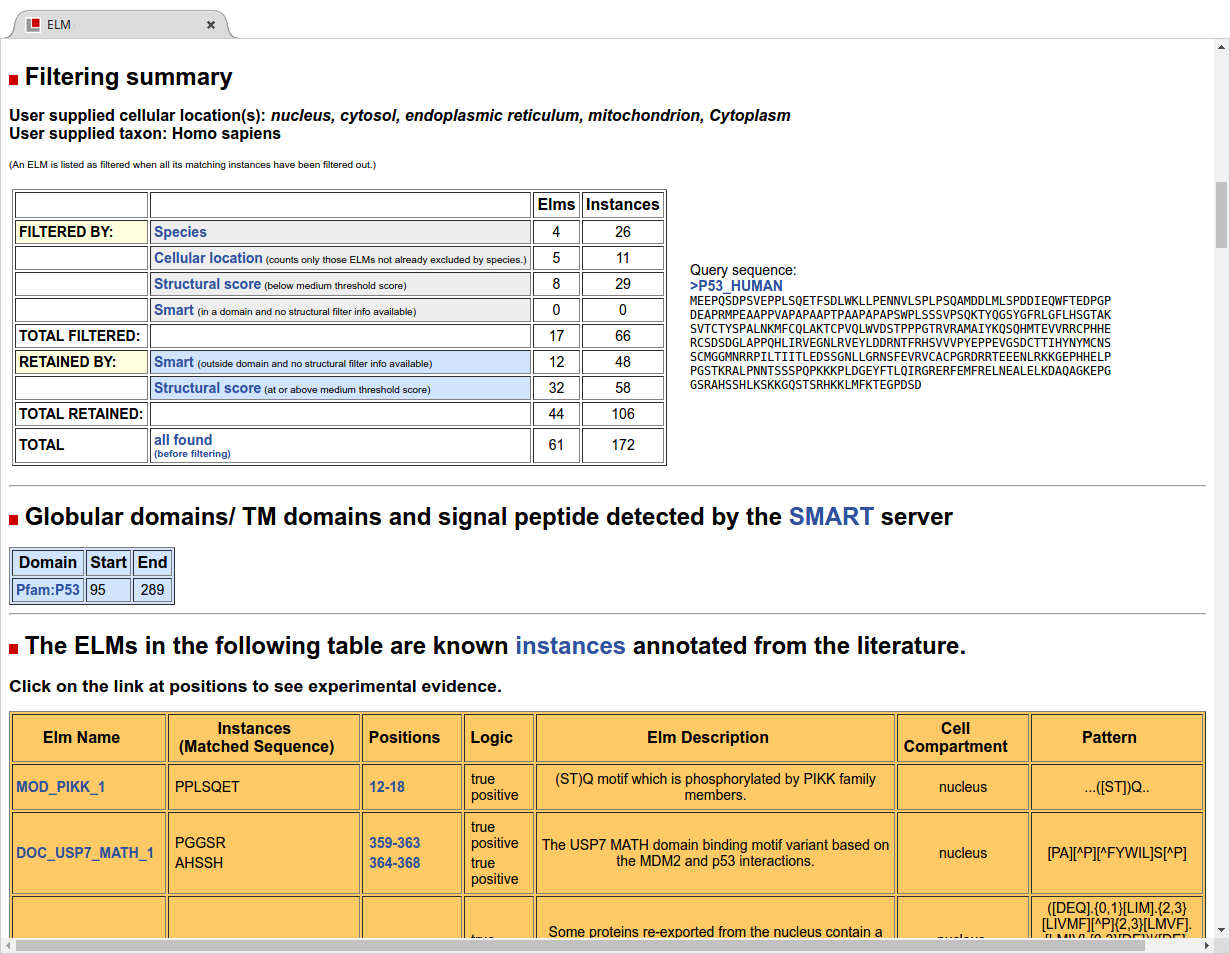
\includegraphics[width=\textwidth]{Figures/predicting_p53/elm_results_alignments_filtering_domains.png}
	\caption{
	This section of the results contains additional details on the
	homologue alignments used to calculate the conservation score,
	filtering results and globular domains.
	}
	\label{fig:predicting_p53_elm_results_alignemnt_filtering_domains}
\end{figure}

\item Scroll down to below the results graphic to find additional information
	on the ELM prediction pipeline's results
	(Fig. \ref{fig:predicting_p53_elm_results_alignemnt_filtering_domains}).
	The first
	section contains links to download or view the multiple sequence
	alignments of homologous proteins used to calculate the conservation
	score. Click on the link ``Click here to enable the multiple sequence
	alignment viewer'' to open the alignment in Jalview (note: this
	requires the Java browser plugin, which might not be available on some
	browsers). Alternatively you can also download the ``alignment'',
	``conservation features'' and ``phosphosite features'' files separately
	to view on a desktop (non-browser) installation of Jalview
	(\cite{19151095}).

	\sdesc{ The search for possible homologues is performed against the
		UniRef90 database, a dataset of protein sequences with less
		than 90 percent identity between any two of them
		\cite{17379688}. It may occur that the BLAST results
		are not finished when the results page is shown: We suggest to
		refresh the page if you see the message ``Either not enough
		data available to calculate a sequence alignment or the
		calculations haven't finished yet''. In some cases it is also
		possible that no homologues will be detected. If you have
		refreshed the page after waiting for more than 3 minutes, this
		is most likely the case.}

\item Scroll down to the section titled ``Filtering Summary'' to view some
	statistics about how many motifs and instances were filtered out
	(Fig.
	\ref{fig:predicting_p53_elm_results_alignemnt_filtering_domains}).
	The first two lines contain information on whether
	and which filters were applied in step 1 of this protocol.
	In this case 4 motifs (elms) representing 26 instances were filtered
	out as they did not occur in \textit{Homo sapies}. An additional 5
	motifs (representing 11 instances) were filtered out becuase they are
	not annotated to the cell compartments automatically filled in on the
	search page (Step 1).
	The next three lines (``SMART'' \& ``Structural score'') show how many
	motifs and instances were not removed by the SMART and Secondary
	structure filters. A total of 42 motifs (representing 106 instances)
	passed the structural filter.

	\sdesc{Note that the graphical summary above does not contain sequences
		filtered out by the ``cell compartment'' and ``taxonomic
		context'' filters. However those filtered out by
		the SMART and Structural scores are shown in the graphic above
		(as gray rectangles).}

\begin{figure}[h!]
	\centering
	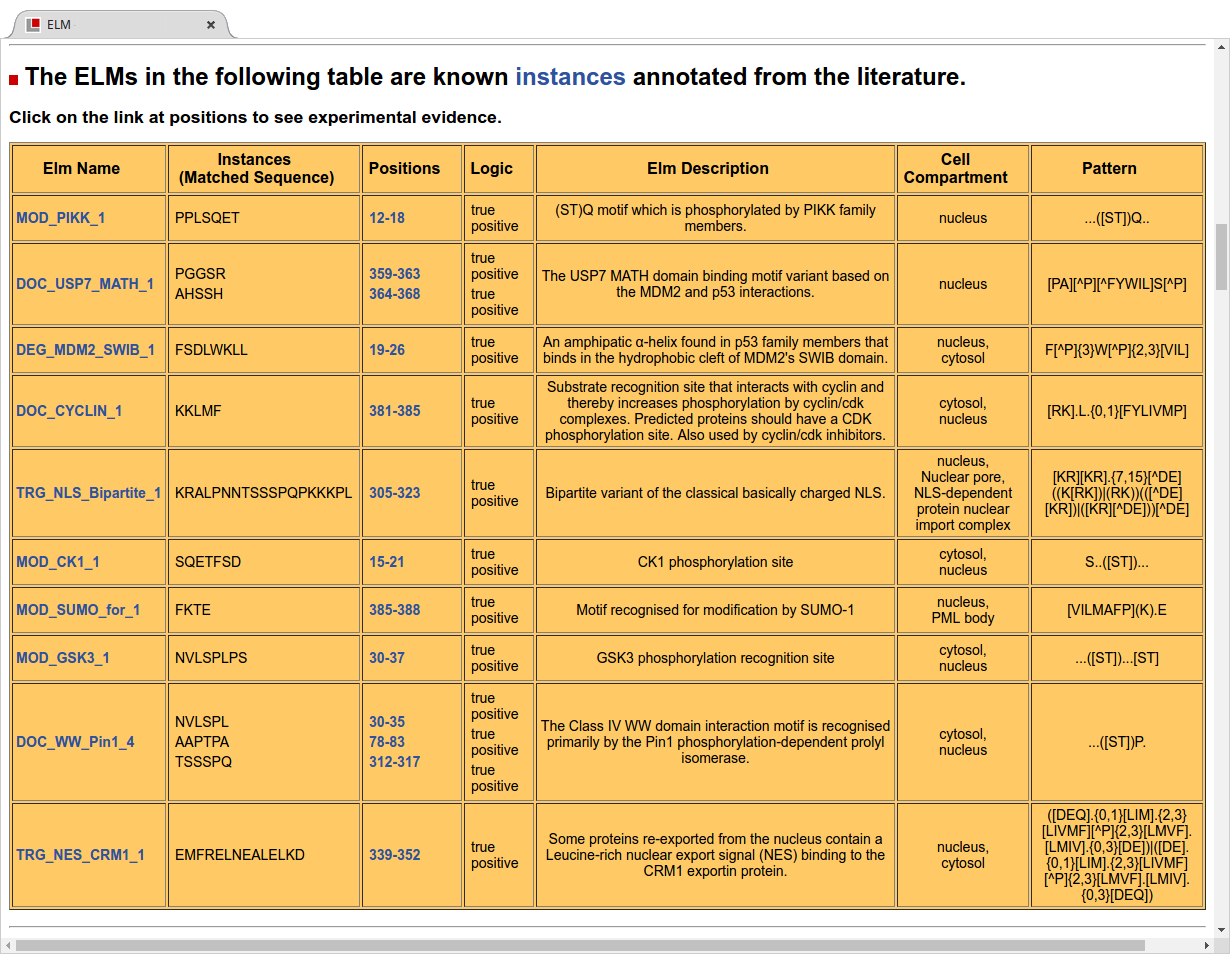
\includegraphics[width=\textwidth]{Figures/predicting_p53/elm_results_known.png} 
	\caption{
		The ELM prediction pipeline section displaying the P53 motifs
		that are ``known'', and have been annotated in the ELM
		database.
	}
	\label{fig:predicting_p53_elm_results_known}
\end{figure}

\item Scroll down to the section with the header ``Globular domains/ TM domains
	and signal peptide detected by the SMART server''
	(Fig. \ref{fig:predicting_p53_elm_results_alignemnt_filtering_domains}).
	This section contains information on which domains were detected by the
	SMART server, and their positions. Clicking on their names will bring
	you to the entry for that domain on the SMART or Pfam homepage.
	In this case the only domains detected is the ``P53'' Pfam domain.

\item On the results page, scroll down to the heading: ``The ELMs in the
	following table are known instances annotated from the literature''
	(\ref{fig:predicting_p53_elm_results_known}).
	This table has details of the motifs and instances which have been
	manually annotated in the ELM database. The columns show each motif
	name, the sequence(s) that matched the motif as well as their starting
	and ending positions and the logic of the annotation followed by a
	short description of each motif, to which cell compartments its has
	been associated, and finally the regular expression of the motif.

\begin{figure}[h!]
	\centering
	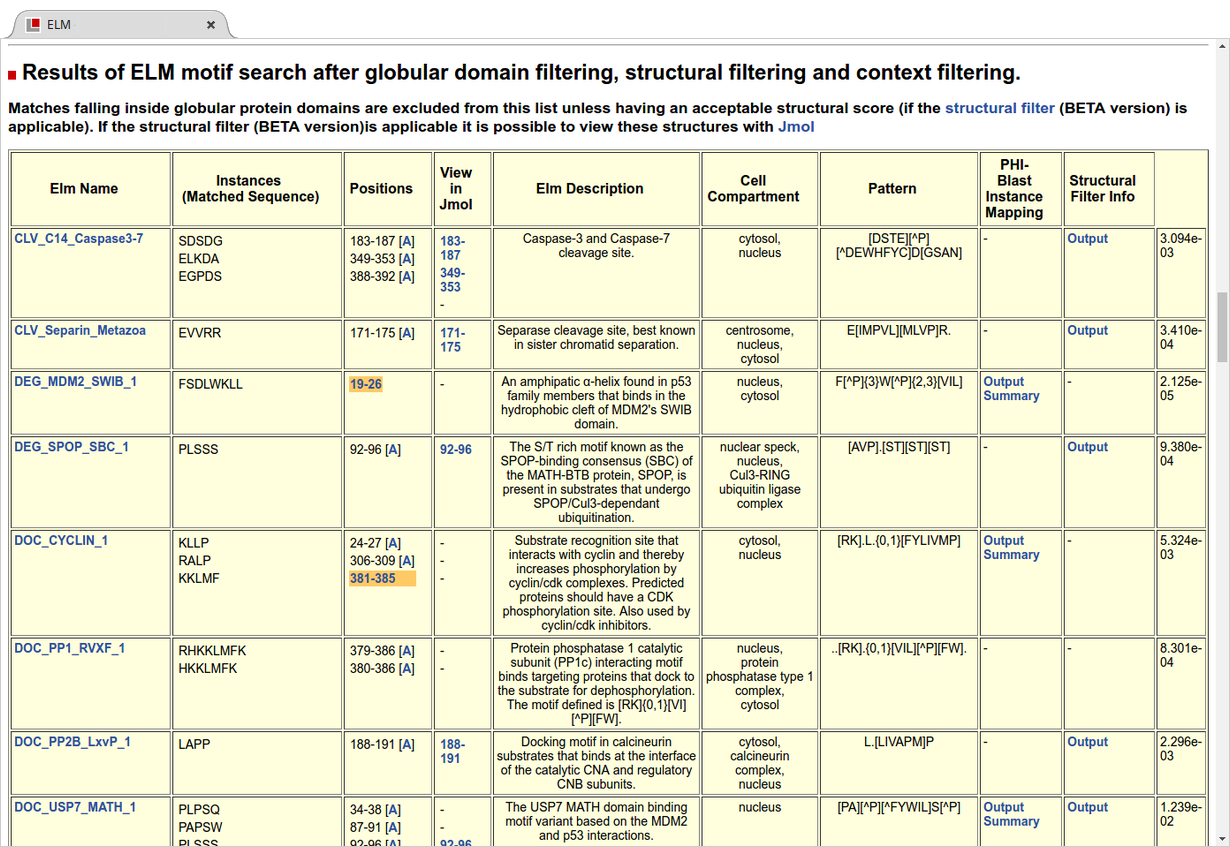
\includegraphics[width=\textwidth]{Figures/predicting_p53/elm_results_motifs.png}
	\caption{
	This table contains the list of motifs detected in the sequence (only
	the top part of the table is shown). These are predictions in the sense
	that the sequence in present, however its is known whether they are
	\emph{bona-fide} motifs which are biologically functional.
	}
	\label{fig:predicting_p53_elm_results_motifs}
\end{figure}

\item Scroll further down to the section title ``Results of ELM motif search
	after globular domain filtering, structural filtering and context
	filtering'' to obtain an overview of all of the motifs and motif
	instances detected
	(\ref{fig:predicting_p53_elm_results_motifs})
	Each of the rows is a ``predicted'' motif: A sequence matching a
	motif's regular expression has been detected that has also passed the
	``structural filter''.
	Each row displays the motif identified, the matching peptide
	sequence and its position. Additional information is shown about the
	motif, its cell compartment and its regular expression. If the motif
	was detected in a homologue, the column ``PHI-Blast Instance
	mapping'' contains a link to the multiple sequence alignment of the
	homologous proteins. If a motif instance has been filtered out 
	by the ``structural filter'', the ``Structural filter info'' column
	contains a link to a page with details on why.
	The last column contains information on the Probability filter: the
	probability reflects the chance to observe this motif in any random
	amino acid sequence (see section \ref{sec:explore_content})

\begin{figure}[h!]
\centering
	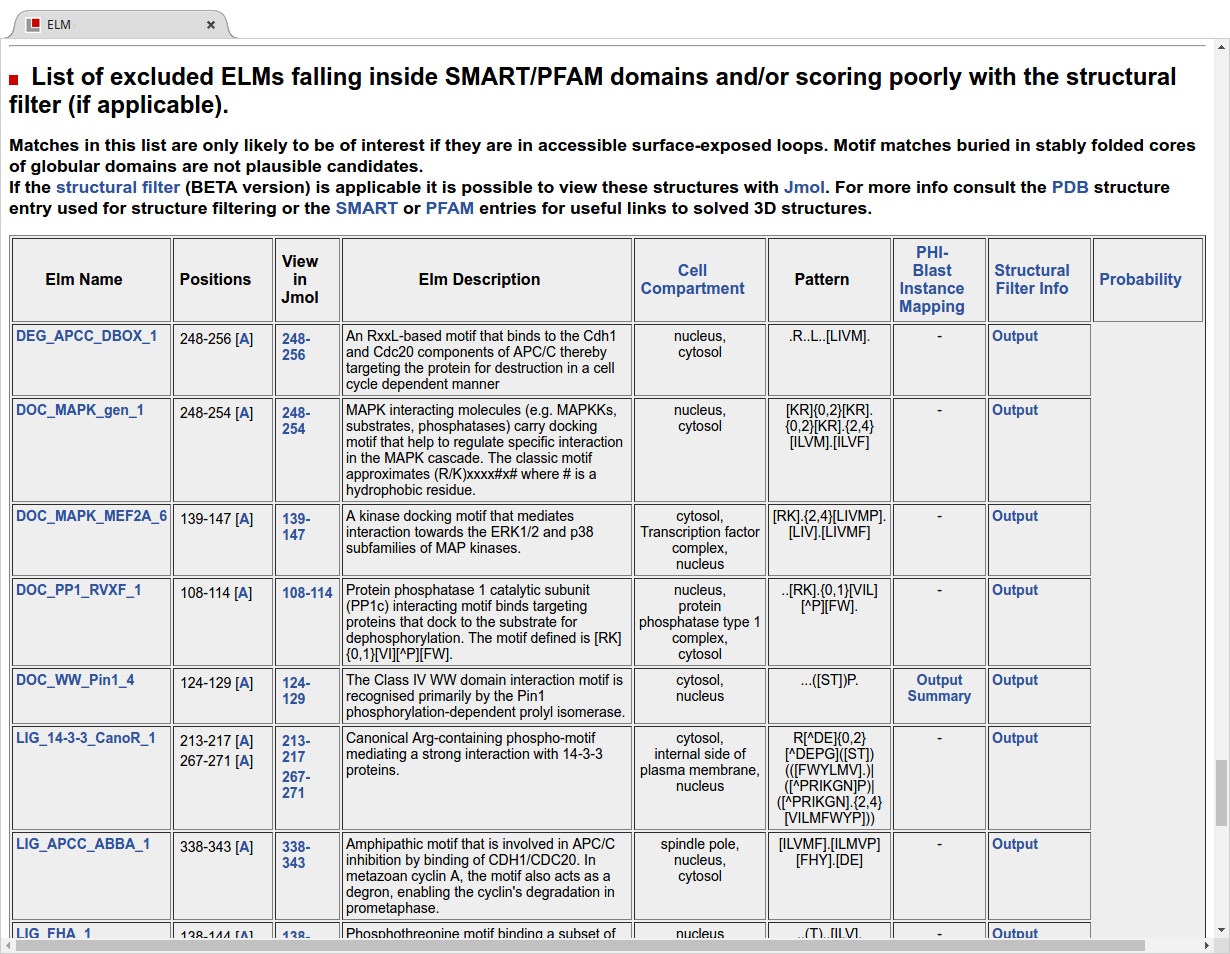
\includegraphics[width=\textwidth]{Figures/predicting_p53/elm_results_motifs_filtered.png}
	\caption{
	This table contains the list of motifs detected in the sequence (only
	the top part of the table is shown) which were excluded by the
	structural filter.
	}
	\label{fig:predicting_p53_elm_results_motifs_filtered}
\end{figure}

\item Scroll further down to the heading ``List of excluded ELMs falling inside
	SMART/Pfam domains and/or scoring poorly with the structural filter (if
	applicable).''
	(Fig.  \ref{fig:predicting_p53_elm_results_motifs_filtered)})
	This table is similar to the one described above, but shows motif
	matches which were rejected by the structural filter.
	
\end{enumerate}
